\section{Pendahuluan}
\subsection{Latar Belakang}
Pada modul ini, kita akan membahas konfigurasi routing static dan routing dinamis pada perangkat
MikroTik. Routing merupakan proses pengiriman data antara dua atau lebih jaringan yang berbeda.
Dalam modul ini, kita akan membahas konsep dasar routing, macam-macam routing statis dan
dinamis, serta langkah-langkah untuk mengkonfigurasi kedua jenis routing ini pada perangkat
MikroTik.\\\\
Sebelum memulai pembahasan routing, penting untuk memahami konsep dasar jaringan dan
subnetting. Jaringan terdiri dari sejumlah perangkat yang terhubung satu sama lain, seperti komputer,
printer, dan perangkat jaringan lainnya. Setiap perangkat dalam jaringan memiliki alamat IP yang
unik.

\subsection{Maksud dan Tujuan}
Mengetahui dan memahami konfigurasi routing static dan routing dinamis pada Mikrotik.

\subsection{Hasil yang diharapkan}
Dapat mengkonfigurasi konfigurasi routing static dan routing dinamis pada Mikrotik dengan
tepat.

%===========================================================%
\section{Tugas Pendahuluan}
\begin{enumerate}
\item Buatlah

%===========================================================%
\section{Alat dan Bahan}
\begin{itemize}[label=$\bullet$, itemsep=-1pt, leftmargin=*]
	\item Buatlah
\end{itemize}

%===========================================================%
\section{Jangka Waktu Pelaksanaan}
Pemahaman dan konfigurasi 1 jam.

%===========================================================%

\section{Proses dan Tahapan Konfigurasi}
%======================PERCOBAAN 1==========================%
\subsection{Wireless Point to Point}
\begin{center}

\textbf{Konfigurasi Router 1}
\begin{enumerate}
	\item Buka aplikasi WinBox pada PC 1 dan lakukan koneksi ke Router 1.\\Neighbors > Refresh > Double click Router yang terdeteksi > Connect
	      \begin{figure}[H]
		      \centering
		      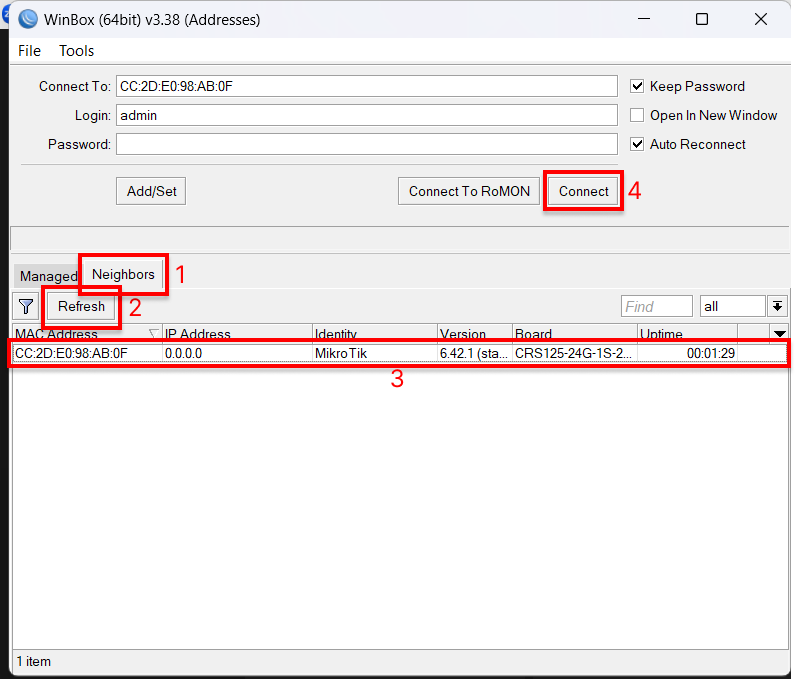
\includegraphics[width=0.8\linewidth]{P1/img/per1/pc1/Step 1.png}
		      \caption{Step 1}
		      \label{fig:Step 1(Per.1 PC1)}
	      \end{figure}
\end{enumerate}

\textbf{Konfigurasi Router 2}
\begin{enumerate}
	\item Buka WinBox dan lakukan koneksi ke Router
	      \begin{figure}[H]
		      \centering
		      \includegraphics[width=0.9\linewidth]{P1/img/per1/pc2/Step 2.png}
		      \caption{Step 2}
		      \label{fig:Step 2(Per.1 PC2)}
	      \end{figure}
\end{enumerate}

\textbf{Pengujian konfigurasi}
\begin{enumerate}
\item Lakukan test ping dari Router 1 ke Router 2
\begin{figure}[H]
	\centering
	\includegraphics[width=0.9\linewidth]{P1/img/per1/pc1/Step 4.png}
	\caption{Step 1}
	\label{fig:Ping Step 1(Per.1 PC1)}
\end{figure}
\end{center}

%======================PERCOBAAN 2==========================%
\subsection{Wireless Point to Multipoint}
\begin{center}

	\textbf{Konfigurasi Router 1}
	\begin{enumerate}
		\item Berikan IP address sesuai dengan cara pengaturan IP address yang benar. Berikan IP address yang berbeda dengan contoh di modul.
		      \begin{figure}[H]
			      \centering
			      \includegraphics[width=0.9\linewidth]{P1/img/per1/pc1/Step 2.2.png}
			      \caption{Step 1}
			      \label{fig:Step 1(Per.2 PC1)}
		      \end{figure}
	\end{enumerate}

	\textbf{Konfigurasi Router 2}
	\begin{enumerate}
		\item Berikan IP address pada interface wlan 1 yang dapat dibuat pada tab IP > Addresses. Berikan IP address sesuai dengan cara pengaturan IP address yang benar. Berikan IP address yang berbeda dengan contoh di modul.
		      \begin{figure}[H]
			      \centering
			      \includegraphics[width=0.9\linewidth]{P1/img/per1/pc2/Step 2.png}
			      \caption{Step 1}
			      \label{fig:Step 1(Per.2 PC2)}
		      \end{figure}
	\end{enumerate}

	\textbf{Pengujian konfigurasi}
	\begin{enumerate}
		\item Lakukan test ping dari Router 1 ke Router 2
		      \begin{figure}[H]
			      \centering
			      \includegraphics[width=0.9\linewidth]{P1/img/per2/pc1/Step 4.png}
			      \caption{Step 1}
			      \label{fig:Ping Step 1(Per.2 PC1)}
		      \end{figure}
	\end{enumerate}

\end{center}

%======================PERCOBAAN 3==========================%
\subsection{Wireless Bridge}
\begin{center}

	\textbf{Konfigurasi Router 1}
	\begin{enumerate}
		\item Buka WinBox dan lakukan koneksi ke Router
		      \begin{figure}[H]
			      \centering
			      \includegraphics[width=0.9\linewidth]{P1/img/per3/pc1/Step 2.png}
			      \caption{Step 2}
			      \label{fig:Step 2(Per.3 PC1)}
		      \end{figure}
	\end{enumerate}

	\textbf{Konfigurasi Router 2}
	\begin{enumerate}
		\item Berikan IP address pada interface wlan1 dan ethernet 2 yang dapat dibuat pada tab IP > Addresses. Berikan IP address sesuai dengan cara pengaturan IP address yang benar. Berikan IP address yang berbeda dengan contoh di modul.
		      \begin{figure}[H]
			      \centering
			      \includegraphics[width=0.9\linewidth]{P1/img/per3/pc2/Step 2.png}
			      \caption{Step 2}
			      \label{fig:Step 2(Per.3 PC2)}
		      \end{figure}
	\end{enumerate}

	\textbf{Pengujian konfigurasi}
	\begin{enumerate}
		\item Lakukan test ping dari PC 1 ke PC 2
		      \begin{figure}[H]
			      \centering
			      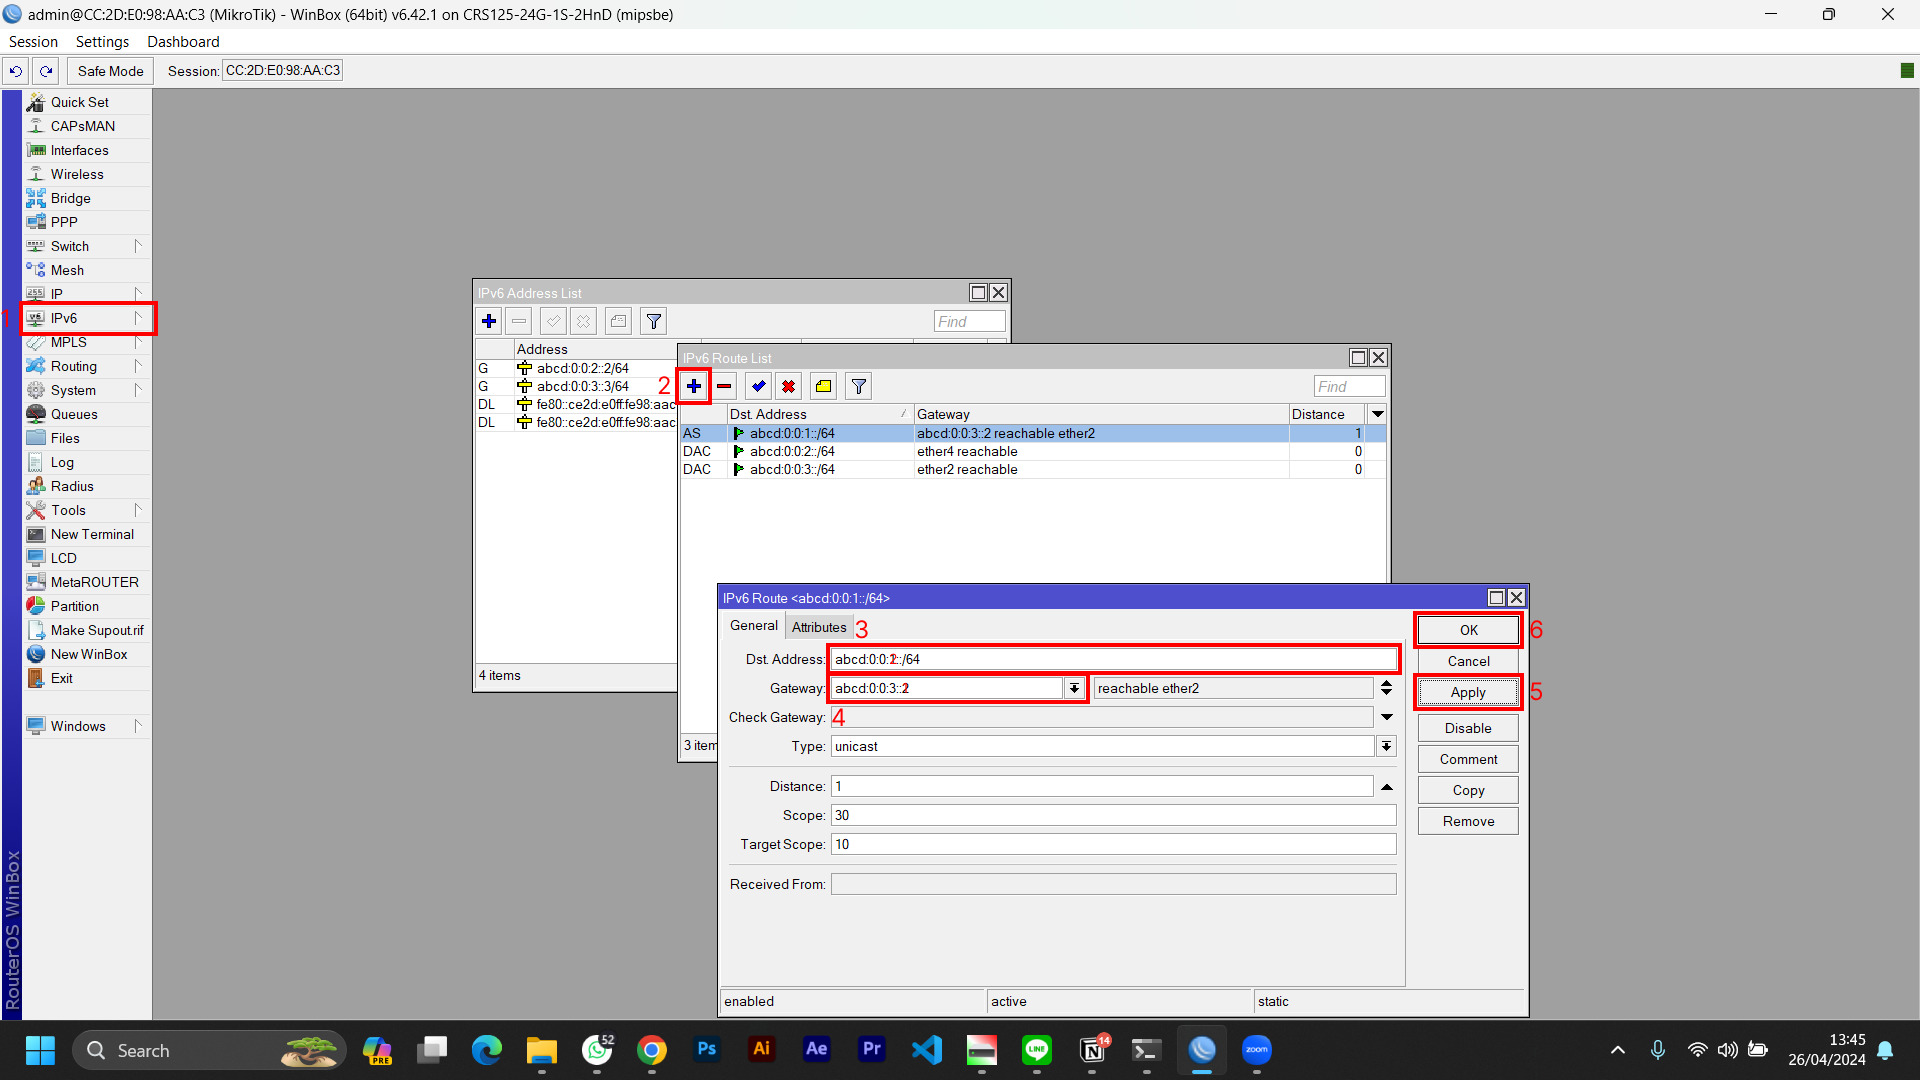
\includegraphics[width=0.9\linewidth]{P1/img/per3/pc1/Step 7.png}
			      \caption{Step 7}
			      \label{fig:Step 7(Per.3 PC1)}
		      \end{figure}
	\end{enumerate}

\end{center}

%===========================================================%
\section{Hasil yang didapat}
Memahami dan mengkonfigurasi koneksi Point to Point, Point to Multipoint dan Wireless
Bridging dengan tepat.

%===========================================================%
\section{Temuan Permasalahan}
Firewall hidup pada Laptop dapat mempengaruhi koneksi wireless tidak terhubung, kalian
bisa menonaktifkan firewall di laptop kalian, tetapi hal ini tidak terjadi di semua perangkat.

%===========================================================%
\section{Kesimpulan}
Dengan memahami dan mengkonfigurasi 3 jenis koneksi pada wireless, kita dapat
mengimplementasikan koneksi wireless dengan tepat sesuai kebutuhan dan kondisi tertentu.
